\let\negmedspace\undefined
\let\negthickspace\undefined
\documentclass[journal]{IEEEtran}
\usepackage[a5paper, margin=10mm, onecolumn]{geometry}

\usepackage{tfrupee} 

\setlength{\headheight}{1cm} 
\setlength{\headsep}{0mm}     

\usepackage{gvv-book}
\usepackage{gvv}
\usepackage{cite}
\usepackage{amsmath,amssymb,amsfonts,amsthm}
\usepackage{algorithmic}
\usepackage{graphicx}
\graphicspath{{figs/}}
\usepackage{textcomp}
\usepackage{xcolor}
\usepackage{txfonts}
\usepackage{listings}
\usepackage{enumitem}
\usepackage{mathtools}
\usepackage{gensymb}
\usepackage{comment}
\usepackage[breaklinks=true]{hyperref}
\usepackage{tkz-euclide} 
\usepackage{listings}
                                    
\def\inputGnumericTable{}                                 
\usepackage[latin1]{inputenc}                                
\usepackage{color}                                            
\usepackage{array}                                            
\usepackage{longtable}                                       
\usepackage{calc}                                             
\usepackage{multirow}                                         
\usepackage{hhline}                                           
\usepackage{ifthen}                                           
\usepackage{lscape}

\begin{document}

\bibliographystyle{IEEEtran}

\title{1.5.13}
\author{EE25BTECH11025 - Ganachari Vishwambhar}

{\let\newpage\relax\maketitle}

\renewcommand{\thefigure}{\theenumi}
\renewcommand{\thetable}{\theenumi}
\setlength{\intextsep}{10pt}


\numberwithin{equation}{enumi}
\numberwithin{figure}{enumi}
\renewcommand{\thetable}{\theenumi}

\textbf{Question}:\newline
Find the ratio in which the $Y$ axis divides the line segment joining the points $\vec{A}\brak{-1,-4}$ and $\vec{B}\brak{5,-6}$. Also find the coordinates of the point of intersection.\\
\textbf{Solution: }\\

\begin{tabular}[12pt]{|c|c|}
\hline
\textbf{Variable}&\textbf{characteristic}\\
\hline
$\vec{C}$&point of intersection of the line segment and y-axis\\
\hline
$x$&x-coordinate of the point $\vec{C}$\\
\hline
$y$&y-coordinate of point $\vec{C}$\\
\hline
$m$&Slope of line segment joining $\vec{A}$ and $\vec{B}$\\
\hline
\end{tabular}\\

Slope of line segment joining $\vec{A}$ and $\vec{B}$:\\
\begin{align}
m=\frac{\brak{-6}-\brak{-4}}{5-\brak{-1}}\\
m=\brak{\frac{-1}{3}}
\end{align}

Equation of the line joining the points $\vec{A}$ and $\vec{B}$ is\\
\begin{align}
\brak{Y-\brak{-6}}=m\brak{X-5}\\
X+3Y=-13
\end{align}

Equation of $Y$-axis is $X=0$

The point of intersection of the given line segment and the $Y$-axis is:\\
\begin{align}
\myvec{1&3\\1&0}\myvec{x\\y}=\myvec{-13\\0}\\
\myvec{x\\y}=\myvec{0\\\brak{\frac{-13}{3}}}
\end{align}

Hence the coordinates of $\vec{C}$ are $\brak{0,\brak{\frac{-13}{3}}}$

The ratio in which the $Y$-axis divides the given line segment is:\\
\begin{align}
    {\frac{AC}{CB}}=\frac{1}{5}
\end{align}
\begin{figure}[h!]
   \centering
   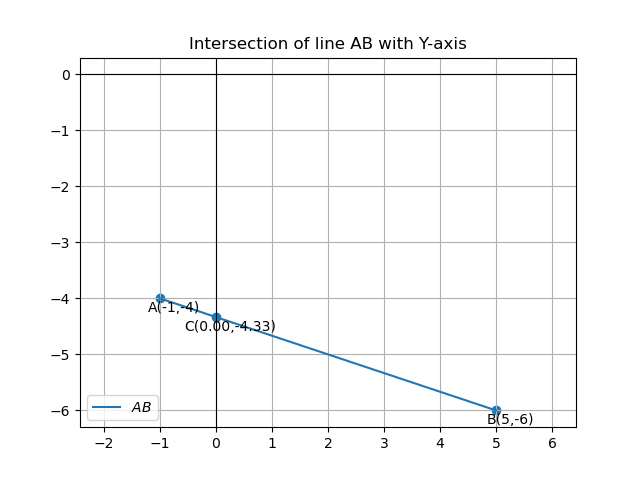
\includegraphics[width=0.7\linewidth]{figs/plot.png}
   \caption{Plot of line segment \textbf{AB}}
   \label{}
\end{figure}
\end{document}  